
%\documentclass[12pt]{amsart}
%\usepackage{geometry} % see geometry.pdf on how to lay out the page. There's lots.
%\geometry{a4paper} % or letter or a5paper or ... etc
% \geometry{landscape} % rotated page geometry

\documentclass[11pt,letter]{article}

%\usepackage[latin1]{inputenc}
\usepackage{epsfig}
\usepackage{amsmath}
\usepackage{mdframed}
%\usepackage{amsfonts}
\usepackage{amssymb}
\usepackage{listings}
\usepackage{booktabs}
\usepackage{setspace}
\usepackage[colorlinks,citecolor=blue]{hyperref}
\usepackage{xcolor}
\usepackage[sort&compress,numbers]{natbib}
%\usepackage{natbibspacing}

\setlength{\oddsidemargin}{.46cm}
\setlength{\evensidemargin}{-0.46cm}
\setlength{\evensidemargin}{0.0cm}
\setlength{\textwidth}{15.5cm}
\setlength{\parskip}{1.0ex plus 0.6ex minus 0.6ex}
\setlength{\parindent}{1.0em} 
\setlength{\textheight}{22.5cm}
\setlength{\topmargin}{-2cm}
\setlength{\footskip}{2cm}
\setlength{\parindent}{0.0cm}

\def\aj{Astron. J.}
\def\apj{Astrophys. J.}
\def\apjl{Astrophys. J. Lett.}
\def\apjs{Astrophys. J. Supp. Ser. }
\def\aa{Astron. Astrophys. }
\def\aap{Astron. Astrophys. }
\def\araa{Ann.\ Rev. Astron. Astroph. }
\def\physrep{Phys. Rep. }
\def\mnras{Mon. Not. Roy. Astron. Soc. }
\def\mmsun{M_\odot}
\def\prl{Phys. Rev. Lett.}
\def\prd{Phys. Rev. D.}
\def\azh{Soviet Astron.}
\def\apss{Astrophys. Space Sci.}
\def\cqg{Class. Quantum Grav.}


\usepackage{mathpazo}
\DeclareMathOperator{\diff}{d\!}
\newcommand{\modot}{M$_\odot$\hspace*{0.05cm}}
\def\apj{Astrophys. Journal}
\def\apjl{Astrophys. Journal Letters}
\def\aap{Astron. Astrophys.}

\setlength{\parskip}{.2cm}

\newcommand{\pd}[2]{\frac{\partial #1}{\partial #2}} 
\newcommand{\pdtwo}[3]{\frac{\partial #1}{\partial #2 \partial #3}} 
\newcommand{\pdtri}[4]{\frac{\partial #1}{\partial #2 \partial #3 \partial #4}} 
\newcommand{\grad}{\vec{\nabla}}
\newcommand{\ddiv}{\vec{\nabla}\cdot}
\newcommand{\intl}{\int\limits}
\newcommand{\msun}{M$_\odot$\ }
\newcommand{\mo}{\mathrm{M}_\odot }
\newcommand{\code}[1]{{\tt #1}}
\newcommand{\todo}[1]{{$\blacksquare$~\textbf{\color{blue}[TODO: #1]}}~$\blacksquare$}
\newcommand{\warn}[1]{{$\blacksquare$~\textbf{\color{red}[WARNING: #1]}}~$\blacksquare$}

% See the ``Article customise'' template for come common customisations

\title{NSE EOS Notes}
\author{Luke Roberts, Ermal Rrapaj, Sanjay Reddy}
\date{} % delete this line to display the current date

%%% BEGIN DOCUMENT
\begin{document}

\maketitle
\tableofcontents

\section{Introduction}
Here we describe the components of an equation of state (EOS) that goes beyond
the single nucleus approximation and naturally transitions to nuclear
statistical equilibrium (NSE).  It is assumed that the bulk free energy is
known, so our model is a generic, phenomenological description of the
non-uniform phase during the nuclear liquid-gas phase transition.  In different
limits, it reduces to the excluded volume model of Hempel, the single nucleus
approximation of Lattimer, or to a simple two charge Gibbs phase construction.  

\section{The free energy}  
Basically, our model assumes a multi-phase medium where each phase bubble --
aside from the exterior bulk -- is constrained to have a fixed neutron and
proton number.  This is a straight forward generalization of LS.  Clearly, a
phase bubble can alternatively thought of as a nucleus.  In the spirit of LS,
our model Helmholtz free energy for nuclear matter is 
\begin{equation}
F = \sum_i^{\textrm{nuclei}} F_i(v_i,n_i,T) + V_o f_{B}(n_{p,o},n_{n,o},T).
\end{equation}
where $f_B$ is the free energy of homogeneous nuclear matter per volume, $n_x$
is the number density of species $x$, $v_i$ is the volume of nucleus (or phase)
$i$, the subscript $o$ denotes nucleons outside of nuclei and corresponds to the
low density phase (at densities below pasta formation).  Here, $V_o = V - \sum v_i \mathcal{N}_i$ is the volume 
not taken up by nuclei.  The total free energy
of phase $i$ is modeled as 
\begin{equation}
F_i = \mathcal{N}_i \left[ v_i f_B(\frac{Z_i}{v_i},\frac{N_i}{v_i},T) 
+ F_{FS}(v_i,Z_i,N_i,n_{p,o},n_{n,o},n_e,T) + T \ln \left(\frac{n_i}{n_Q A_i^{3/2}}\right) 
- T + E_{0,i}\right],
\end{equation}   
where $\mathcal{N}_i = V n_i$, $n_Q = (m_n T / 2 \pi)^{3/2}$, $n_e$ is the
number density of uniform electrons, and $F_{FS}$ is the free energy
contribution from finite size effects such as surface tension and Coulomb
corrections.  Shell and pairing effects can be included through $E_{0,i}$.  If
we assumed there were a single nucleus (i.e. only one $N_i$ and $Z_i$) and
allowed these neutron and proton number of the nucleus to vary, we arrive at the
model free energy used in LS.  

\subsection{Minimization of the Free Energy}
\label{sec:minimization}
To find the thermodynamic state of the system, we must minimize our free energy
with respect to the free parameters in our model subject to the constraints of
total neutron number, proton number, and volume conservation.  These constraints
are written as \begin{eqnarray}
\sum \mathcal{N}_i Z_i + Z_o = Z \\
\sum \mathcal{N}_i N_i + N_o = N \\
\sum \mathcal{N}_i v_i + V_o = V, 
\end{eqnarray}
where $Z_o = n_{p,o} V_o$ and $N_o = n_{n,o} V_o$.  Choosing $\mathcal{N}_i$ and
$v_i$ as our independent variables gives the relations \begin{eqnarray} 
Z_i + \frac{\partial Z_o}{\partial \mathcal{N}_i} = 0, \,\, \,\,
N_i + \frac{\partial N_o}{\partial \mathcal{N}_i} = 0 \\
v_i + \frac{\partial V_o}{\partial \mathcal{N}_i} = 0, \,\, \,\,
\mathcal{N}_i + \frac{\partial V_o}{\partial v_i} = 0
\end{eqnarray}
and results in the system of equations 
\begin{eqnarray}
\label{eq:dFdN}
&&\frac{\partial F}{\partial \mathcal{N}_i} = v_i f_{B,i} + F_{FS,i} 
+ \mu_{K,i} + E_{0,i} - Z_i \mu_{p,o} - N_i \mu_{n,o} + v_i P_o  = 0 \\
\label{eq:dFdv}
&&\frac{\partial F}{\partial v_i} = \mathcal{N}_i 
\left(- P_{B,i} - P_{FS,i} + P_{o} \right) = 0 \\ 
&&\sum Z_i n_i + \left(1-\sum v_i n_i \right) n_{p,o} = n_p = n_e \\
&&\sum N_i n_i + \left(1-\sum v_i n_i \right) n_{n,o} = n_n,
\end{eqnarray}
where we have defined $\mu_{K,i} = T \ln (A_i^{-3/2} n_i/n_Q)$, 
$P_{B,i} = -\partial (v_i f_{B,i}) / \partial v_i$, and 
$P_{FS,i} = -\partial (F_{S,i}) / \partial v_i$.


\subsection{Connection to NSE} 
Here we discuss the physics of NSE for an ensemble of non-interacting nuclei and
show how a similar formulation results from our multi-nucleus Gibbs
construction.  

\subsubsection{Basic NSE} 
For a reaction $i \leftrightarrow j + k$, it is easy to show that the principle
of detailed balance implies that 
\begin{equation}
\mu_i = \mu_j + \mu_k 
\end{equation} 
holds when the forward rate balances the backward rate.  When all strong
interactions are in equilibrium with their inverses, invoking detailed balance
for all of the reactions implies that 
\begin{equation}
\mu_i = N_i \mu_n + Z_i \mu_p. 
\end{equation} 
where $N_i$ is the number of neutrons and $Z_i$ is the number of protons in a
nucleus of species $i$.
This of course implies that if the neutron and proton number densities are
known, the number densities of all other species in the medium are known.
Assuming that the heavy nuclei obey Boltzmann statistics (i.e. $\mu_i = m_i + T
\ln \left[n_i/(G_i n_Q)\right]$ gives 
\begin{equation}
\label{eq:nse1}
n_i = A_i^{3/2} G_i(T) n_Q \exp\left(\left[Z_i \mu_p + N_i \mu_n
- m_i \right]/T\right), 
\end{equation} 
where $G_i$ is the temperature dependent internal partition function of species
$i$.  When neutrons and protons also obey Boltzmann statistics, the number
density can be expressed as 
\begin{equation} 
n_i = \frac{A_i^{3/2} G_i(T)}{2^{A_i}n_Q^{A_i-1}}  n_n^{N_i} n_p^{Z_i}
\exp(BE_i/T), 
\end{equation} 
where $BE_i$ is the binding energy and $G_i$ is the internal partition function
of species $i$.  

Rather than being given the free proton and neutron densities, we often
only know the total neutron and proton densities.  In that case the equations of
neutron and proton number conservation must be solved as functions of the free
proton and neutron number densities
\begin{eqnarray}
\label{eq:nse2}
&&n_{n,o} + \sum_i^\textrm{nuclei} N_i n_i(n_{n,o}, n_{p,o}) = n_n, \\
\label{eq:nse3}
&&n_{p,o} + \sum_i^\textrm{nuclei} Z_i n_i(n_{n,o}, n_{p,o}) = n_p.
\end{eqnarray}  

The equations of NSE can also be derived by writing minimizing the free energy of a 
multi-component gas subject to the constraints of neutron and proton number
conservation.  The free energy is just 
\begin{equation}
F_{NSE} = V f_B(n_{p,o}, n_{n,o}, T) +  
\sum^{\textrm{nuclei}}_i \mathcal{N}_i \mathrm{f}_i(\mathcal{N}_i/V, T), 
\end{equation} 

where $V$ is the total volume of the system, $\mathcal{N}_i$ is the total
number of particles of species $i$, and 
\begin{equation}
\mathrm{f}_i = m_i + T \ln \left[\frac{\mathcal{N}_i}{V G_i(T)} 
\left(\frac{2 \pi \hbar^2}{m_i T} \right)^{3/2}  \right] - T
\end{equation}
is the specific free energy of species $i$. \warn{We need to be careful about
including the rest mass in the free energy,  the Skyrme output does not include
it so the nucleon binding energies should come in.  This needs to be cleaned up
both in the notes and in the code (although the code is currently consistent)}
The NSE equations (equations \ref{eq:nse1}, \ref{eq:nse2}, and \ref{eq:nse3})
result if this free energy is minimized with respect to the $\mathcal{N}_i$
while maintaining fixed total neutron number, proton number, and volume (similar
to the procedure in section \ref{sec:minimization}).  

\subsubsection{NSE with Excluded Volume Correction}
A slightly more complicated for nuclei in a medium takes into account that the nuclei
take up volume.  The nuclei can exist in the whole volume, but neutrons and protons 
can only exist in the volume not taken up by nuclei.  The free energy for this system
can be written as 
\begin{equation}
F_{EV} = \sum_i^{\textrm{nuclei}} V f_i(\mathcal{N}_i/V, T) 
+ \left (1 - \sum_i^{\textrm{nuclei}}\mathcal{N}_i v_i\right) V \left[f_n + f_p\right].
\end{equation}
Minimizing this free energy results in a very similar set of equations to the NSE 
equations, but with a correction term to the number density of species $i$ because of 
the energetic cost of excluding nucleons from its volume 
\begin{equation}
n_{i,EV} = A_i^{3/2} G_i(T) n_Q \exp\left(\left[Z_i \mu_p + N_i \mu_n - m_i - v_i(P_n + P_p) \right]/T\right).
\end{equation} 

\subsubsection{Relation of Multi-nucleus Gibbs to NSE}
The constraint equations for our model free energy bear a strong resemblance 
to the excluded volume NSE equations (by construction).  This can be seen by recasting 
equation \ref{eq:dFdN} to 
\begin{equation}
n_i = A_i^{3/2} n_Q \exp(Z_i (\mu_{p,o} - m_p) + N_i (\mu_{n,o} - m_n) + \tilde B_i - v_i P_o),
\end{equation}
where 
\begin{equation}
\tilde B_i(v_i, n_{p,o}, n_{n,o}, T) = 
 Z_i m_p + N_i m_n - v_i f_{B,i} - F_{FS,i} - E_{0,i}.
\end{equation}
We can also see that equation \ref{eq:dFdv} is independent of $\mathcal{N}_i$ 
when $n_i$ is non-zero.  This allows us to express the nuclear volume as a 
function of only the properties of the external medium, $v_i = v_i(n_{p,o},
n_{n,o}, T)$, so that $\tilde B_i = \tilde B_i(n_{p,o}, n_{n,o}, T)$ is just 
an external density dependent binding energy for species $i$.  For some choices 
of the properties of the external medium, the pressure equilibrium conditions 
cannot be met for any volume.  This just implies that $n_i$ must be zero, which 
also provides a solution to equation \ref{eq:dFdv}.  When solutions are admitted, 
the expression for the number density of species $i$ can be further massaged to look like standard NSE by expressing the thermal average 
of the excitation energy above the ground state as 
\begin{equation}
\langle E^* \rangle = T \frac{d \ln G}{d \ln T},
\end{equation} 
where $G(T)$ is the internal partition function of the gas and $E^*$ is the 
excitation energy above the zero temperature ground state.  To get the 
internal partition function outside the exponential as would be the case in 
NSE, we must make the identification $ G_i = \exp(d \ln G/ d\ln T)$.  
\todo{This probably should reduce to something like a fermi gas model for the 
level density.  Check if this is in fact the case.}

When the outside densities are low, $P_o$ is negligible and the second
constraint equation results in \begin{equation}
P_{B,i} + P_{FS,i} = 0.
\end{equation} 
As long as the finite size term is not strongly affected by the exterior medium
(which is expected at low densities), this equation only depends on $v_i$.
Therefore, it just determines the volume of nucleus $i$ in vacuum, and thereby
its total energy and entropy.  Combined with the proton and neutron density 
constraint equations, this results in the excluded volume NSE equations employed 
by Hempel, for instance.  Further assuming that $\sum v_i n_i$ and $v_i P_o$ are 
negligible, which is a very good approximation at low density, results in the
standard equations for low density NSE.

\subsection{Connection to Gibbs Phase Equilibrium}
The Gibbs phase construction assumes there are no surface effects and that the
phase bubbles are stationary.  Employing these two approximations forces us to
set $E_{FS,i}$ and $\mu_{K,i}$ to zero (or assume they are negligible).  Our
constraint equations are then \begin{eqnarray}
n_i P_{B,i} = n_i P_o \\ 
v_i f_{B,i} + E_{0,i} =  Z_i \mu_{p,o} + N_i \mu_{n,o} - v_i P_o.
\end{eqnarray}
The relation $P_B = n_p \mu_p + n_n \mu_n - f_B$ (which holds for 
homogeneous matter) can then be employed to recast
the constraints as \begin{eqnarray}
n_i P_{B,i} = n_i P_o \\ 
Z_i \left(\mu_{p,i} - \mu_{p,o}\right) + N_i \left(\mu_{n,i} - \mu_{n,o}\right) = 0\\
\end{eqnarray}
These equations are either satisfied by nucleus $i$ when it's density is zero or
when it satisfies the Gibbs phase equilibrium conditions.  Since there is no
difference between different nuclei with the same $Y_p$ because there is are no
finite size effects, this will just look like a two phase construction.    

\subsection{Connection to the Single Nucleus Approximation} 
\todo{Write down constraint equations with single nuclear species with N and Z 
allowed to vary.}

\section{Thermodynamic Quantities} 
The pressure is given by 
\begin{equation}
P = P_o + \sum n_i \left[ T + \frac{\partial F_{FS,i}}{\partial \ln n_e} 
+ u_o \frac{\partial F_{FS,i}}{\partial \ln n_{p,o}} 
+ u_o \frac{\partial F_{FS,i}}{\partial \ln n_{n,o}} \right]  
\end{equation}
where $\frac{\partial \square }{\partial \text{ln}n_q } \equiv n_q \frac{\partial \square }{\partial n_q }$, 
and the entropy is given by 
\begin{equation}
s = u_o s_{B,o} + \sum n_i \left(S_{B,i} + \frac{5}{2} - \frac{\mu_{K,i}}{T} 
- \frac{\partial F_{FS,i}}{\partial T}\right).
\end{equation}
The chemical potentials are 
\begin{eqnarray}
&& \mu_p = \mu_{p,o} + \sum_i \frac{n_i}{u_0} \frac{\partial F_{FS,i}}{\partial n_{p,o}}, \\
&& \mu_n = \mu_{n,o} + \sum_i \frac{n_i}{u_0} \frac{\partial F_{FS,i}}{\partial n_{n,o}}.
\end{eqnarray}
I think the finite size correction should be there, but this bears double
checking.  The LS model would predict them to be zero, since their expressions for
$F_{FS}$ are independent of the external densities.  In any case, these 
corrections should always be quite small for nuclei.  They can potentially be 
large for voids.

\section{Model for Finite Size Effects}
\subsection{Coulomb Corrections} 
We currently employ the Wigner-Seitz approximation to Coulomb corrections.  In
principle more complicated models could easily be used.  The volume of a charge
neutral spherical cell containing a nucleus of charge $Z_i$ is 
\begin{equation} 
v_{WS,i} = \frac{Z_i - v_i n_{p,o}}{n_e - n_{p,o}}
\end{equation}
and the fraction of this volume filled by the nucleus is 
\begin{equation}
u_i = v_i/v_{WS,i} = \frac{n_e - n_{p,o}}{n_{p,i} - n_{p,o}}. 
\end{equation} 
The total Coulomb contribution to the free energy for a single nucleus is then
given by
\begin{equation}
F_{C,i}(v_i, n_{p,o}, n_e) = \frac{3\alpha}{5 r_i} \left(Z_i - v_i n_{p,o}\right)^2 
\mathcal{D}(u_i),
\end{equation} 
where $\mathcal{D}(u) = 1 - 3/2 u^{1/3} + u/2$.  This expression is valid wether
the exterior phase is low or high density and is applicable when calculating
voids.  Derivatives of this are also required 
\begin{eqnarray}
&& \pd{F_{WS,i}}{\ln n_e} = F_{WS,i} \frac{\mathcal{D}'}{\mathcal{D}}
\pd{u_i}{\ln n_e} \\
&& \pd{F_{WS,i}}{\ln n_{p,o}} = F_{WS,i} \frac{\mathcal{D}'}{\mathcal{D}}
\pd{u_i}{\ln n_{p,o}} - v_i \frac{F_{WS,i}}{Z_i - v_i n_{p,o}}\\
-P_{C,i} &=&  \pd{F_{WS,i}}{v_i} = \frac{F_{WS,i}}{v_i} 
\left[ \frac{\mathcal{D}'}{\mathcal{D}}  \pd{u_i}{\ln v_i} 
- \frac{2n_{p,o}}{n_{p,i} - n_{p,o}} - \frac{1}{3} \right].
\end{eqnarray}
  
\subsection{Surface Tension}
\todo{Come up with a decent surface tension prescription}

\section{Dealing with nuclear inversion}
\todo{Not sure how to deal with it smoothly} 

\section{Numerics}
\todo{Write up what you are doing} 
\subsection{Gibbs Phase Equilibrium Solver}
\subsection{NSE Solver}
The NSE solver and equation of state are found in the file \texttt{src/EquationsOfState/EOSNSE.hpp}.  As was shown above, standard NSE, excluded volume NSE, and our model free energy share a very similar form.  Therefore, a generic NSE solver with excluded volume corrections has been implemented.  It takes a vector of nuclear species that all inherit from the class \texttt{NucleusBase}.  For a given exterior state, these nuclei can return their binding energy, their internal partition function \todo{implement the partition function for generality}, and their volume.  This implies that the NSE solver should be agnostic about what type of nuclei are being passed to it.  Often, it is hard to find a solution to the NSE equations when the composition is dominated by nuclei.  To increase the range over which the solver converges, we use a trick where we turn on the binding energies and volumes of the nuclei as if they were a perturbation.  The number densities then are given by 
\begin{equation}
n_{i} = A_i^{3/2} G_i(T) n_Q \exp\left(\left[Z_i (\mu_p - m_p) + N_i (\mu_n - m_n) 
- \lambda_B B_i - \lambda_v v_i P_o \right]/T\right).
\end{equation}
A solution can easily be found when the $\lambda$s are zero, and then they can be slowly increased to find a solution to our actual system of equations.   There also seem to be problems when the neutrons and protons are assumed to be an interacting gas.  This results in the chemical potentials decreasing with increasing density and prevents a solution from being found.  Currently, it is unclear to me why this is the case. \todo{Understand why this is the case.}

\begin{figure}[t]
\centering
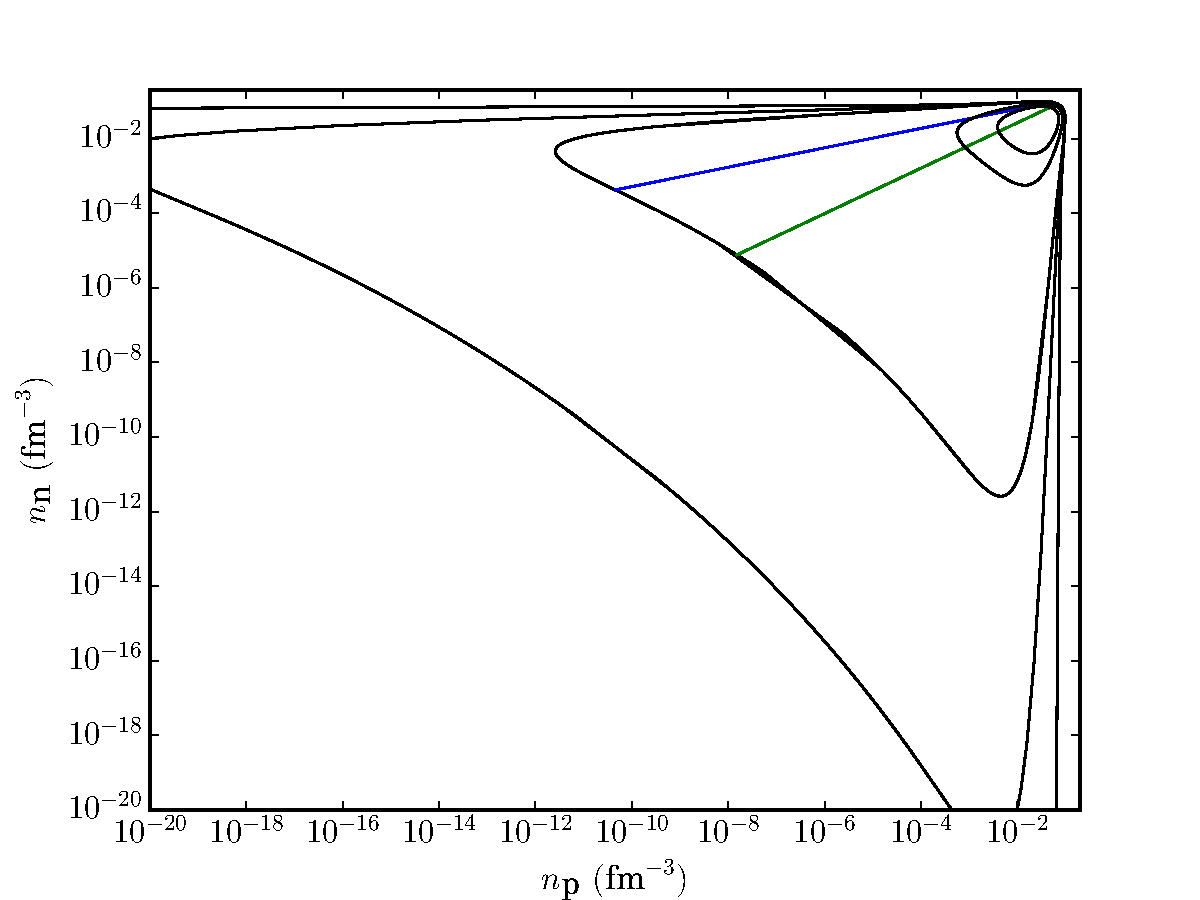
\includegraphics[width=0.9\textwidth]{PhaseBoundaryDensity.pdf}
\vspace*{-0.35cm}
\caption{ Phase boundaries for a variety of temperatures with LS Skyrme.}
\vspace*{-0.7cm}
\end{figure}

\section{Uniform Matter Thermodynamics}
This section deals with the various relationships between the thermodynamic potentials and their derivatives in the framework of uniform matter.
The set of independent parameters is given by $(V,N,Y_i,T)$.
In homogeneous matter, $\mathcal{E}=T\mathcal{S} -P+ \mu_i n_i,\ \mathcal{F} =\mathcal{E} - T\mathcal{S} = -P + \mu_i n_i$.
For constant volume calculations, the indpendent set of parameters becomes 
$(n,Y_i,T)$ and the first law of thermodynamics can be written
as follows,
\begin{equation}
 \begin{split}
  d\mathcal{E}&=Td\mathcal{S}+\mu_i d n_i,\ \ d\mathcal{F} = -\mathcal{S}dT+\mu_i d n_i,\ dP = S dT + n_i d\mu_i\\
 \end{split}
\end{equation}
where, $ \mathcal{S}= S/V,\ n_i=N_i/V,\ n = \sum_i n_i, s= S/N = \mathcal{S}/n,\ f= F/N=\mathcal{F}/n$ and when taking partial derivatives, all other 
independent parameters are kept constant.
Then, $ \mu_i =\partial_{n_i}\mathcal{F},\  \mathcal{S}=-\partial_{T}\mathcal{F}=\partial_T P, \ \mu_i = \partial \mu_i P$.
In practice it is more convenient to work with the following set of parameters, $\mu=\mu_n-\mu_p,\ Y = Y_n-Y_p$ where,$1 = Y_n+Y_p$:
\begin{equation}
 \begin{split}
  &d\mathcal{E}=Td\mathcal{S}+\mu d n,\ \ d\mathcal{F} = -\mathcal{S}dT+\mu d n,\ dP = S dT + n d\mu\\
  &\mu =\partial_{n}\mathcal{E}=\partial_{n}\mathcal{F},\  \mathcal{S}=-\partial_{T}\mathcal{F}=\partial_T P, \ n = \partial \mu P
 \end{split}
\end{equation}

The $1^{st}$ order partial derivatives of $f$ with respect to $(n,Y,T)$ can be found:
\begin{equation}
 \begin{split}
  &\partial_{n}f=-\mathcal{F}/n^{2} +\partial_{n}\mathcal{F}/n= (-\mathcal{F} + \mu n )/n^2=P/n^2\\
  &\partial_{Y} f = \frac{\partial \mathcal{F}}{n \partial Y}=\partial_{n}\mathcal{F}=\mu \\
  &\partial_Tf= \partial_T \mathcal{F}/n =-s\\
 \end{split}
\end{equation}
So,
\begin{mdframed}
\begin{equation}
 \begin{split}
  &\partial_{n}f=P/n^2, \  \partial_{Y} f =\mu, \  \partial_Tf=-s\\
 \end{split}
\end{equation} 
\end{mdframed}
And the 1$^{st}$ law of thermodynamics for the pressure, $dP = S dT + n d\mu$, with $(n,T,Y)$ as independent parameters:
\begin{equation}
 \begin{split}
  \partial_n P =&n \partial_n \mu\\
  \partial_T P =&S = n s+\partial_T \mu\\
  \partial_Y P =&n \partial_Y \mu 
 \end{split}
\end{equation} 
The $2^{nd}$ order mixed partial derivatives give thermodynamic relations among $(P,\mu,s)$:
\begin{equation}
 \begin{split}
  \partial_{Tn}f=\partial_{nT}f \rightarrow -\partial_{n}s=&\partial_TP/n^2\\
  \partial_{TY}f=\partial_{YT}f \rightarrow \partial_T\mu=&-\partial_Ys\\
  \partial_{Yn}f=\partial_{nY}f \rightarrow \partial_n\mu=&\partial_YP/n^2
 \end{split}
\end{equation}
Combining the 2 set of identities above:
\begin{equation}
 \begin{split}
  -\partial_{n}s=\partial_TP/n^2=(n s+\partial_T \mu)/n^2=&s/n\partial_T \mu/n^2=s/n-\partial_Ys/n^2\leftrightarrow\\
  s=&\partial_Ys/n-n\partial_ns\\
 \end{split}
\end{equation}
Also,
\begin{equation}
 \begin{split}
 \partial_T P =& n s+\partial_T \mu \leftrightarrow \\
  \partial_{YT}f=&n^2\partial_{nT}f+n\partial_{T}f
 \end{split}
\end{equation}
The remaining $2^{nd}$ order partial derivatives:
\begin{equation}
 \begin{split}
 \partial_{nn} f =&\partial_n (P/n^2) =\partial_n P/n^2 - 2 P/n^3\\
  =&\partial_{\{nY\}}f/n - 2 \partial_{n}f/n\\
  \partial_{YY}f=&\partial_{Y}\mu\\
  =&\partial_{Y}P/n\\
  =&n\partial_{nY}f\\
  \partial_{TT}f=&-\partial_Ts
 \end{split}
\end{equation}
Since all mixed partial derivatives should be equal under permutations of the order of taking the derivatives, for higher order derivatives
all possible permutations will be denoted by $\{\}$. 
For instance, all mixed derivatives from $T,n,Y$ will be denoted by $\partial_{\{YTn\}}f$.
%So,
%\begin{equation}
% \begin{split}
 % &\partial_{nn} f  =\partial_n P/n^2 - 2 P/n^3=\partial_n \mu /n- 2 \partial_{n}f/n = \partial_{Yn} f /n- 2 \partial_{n}f/n\\
 % &\partial_{nT}f=\partial_T P/n^2 =  s/n+\partial_T \mu/ n^2 = -\partial_{T}f/n+\partial_{YT} f/n^2\\
 % &\partial_{nY} f=\partial_Y P/n^2 = \partial_Y \mu /n = \partial_{YY} f /n 
 %\end{split}
%\end{equation}

Thus, at $2^{dn}$ order, there are only 3 independent partial derivatives and the rest can be calculated from them:
\begin{mdframed}
\begin{equation}
 \begin{split}
 \partial_{YY}f=&n\partial_{\{nY\}}f=n^2\partial_{nn}f+2n\partial_n f\\
  \partial_{\{YT\}}f=&n^2\partial_{\{nT\}}f+n\partial_{T}f\\
 \end{split}
\end{equation}
\end{mdframed}
\begin{mdframed}
\begin{equation}
 \begin{split}
  &\partial_{\{nY\}}f= \partial_n P/n = \partial_n \mu  = \partial_Y P /n^2 = \partial_Y \mu /n \\
  &\partial_{\{nT\}}f=s/n+\partial_T\mu/n^2=s/n-\partial_Ys/n^2=\partial_T P/n^2=-\partial_n s\\
  &\partial_{TT} f =-\partial_T s\\
 \end{split}
\end{equation}
\end{mdframed}
All $3^{rd}$ order derivatives based on $\partial_{TT}f$:
\begin{equation}
 \begin{split}
  \partial_{TTT}f=&-\partial_{TT}s\\
  \partial_{\{TTn\}}f=&\partial_{\{TTY\}}f/n^2-\partial_{TT}f/n\\
  =&-\partial_{\{Tn\}}s=\partial_Ts/n+\partial_{TT}\mu/n^2 = \partial_Ts/n-\partial_{YT}s/n^2=\partial_{TT}P/n^2\\ 
 \end{split}
\end{equation}
All remaining $3^{rd}$ order derivatives based on $\partial_{nT}f$:
\begin{equation}
 \begin{split}
  \partial_{\{nnT\}}f=&\partial_n \big[ \partial_{\{YT\}}f/n^2-\partial_{T}f/n\big]\\
  =&\partial_{\{nTY\}}f/n^2-2\partial_{\{YT\}}f/n^3-\partial_{\{nT\}}f/n+\partial_{T}f/n^2\\
  =&\partial_{\{nTY\}}f/n^2-3\partial_{\{nT\}}f/n+2\partial_{T}f/n^2\\
  =&\partial_{\{Tn\}}P/n^2-2\partial_{T}P/n^3=-\partial_{nn}s\\
  =&\partial_{n}s/n-s/n^2+\partial_{Tn}\mu/n^2-2\partial_{T}\mu/n^3=\partial_{n}s/n-s/n^2-\partial_{\{Yn\}}s/n^2+2\partial_{Y}s/n^3\\
  =&3\partial_Ys/n^3-2s/n^2-\partial_{\{Yn\}}s/n^2
 \end{split}
\end{equation}
All remaining $3^{rd}$ order derivatives based on $\partial_{nY}f$:
\begin{equation}
 \begin{split}
  \partial_{\{YYn\}}f=&\partial_{YYY}f/n=n\partial_{\{nnY\}}f+\partial_{\{nY\}}f=n^2\partial_{nnn}f+4n\partial_{nn}f+2\partial_{n}f\\
  \partial_{\{nnY\}}f=&\partial_{nY}P/n=\partial_{YY}P/n^2=\partial_{nY}\mu=\partial_{YY}\mu/n\\
 \end{split}
\end{equation}
Thus, at $3^rd$ order there are 4 independent partial derivatives:
\begin{mdframed}
\begin{equation}
 \begin{split}
  &\partial_{\{TTn\}}f=\partial_{\{TTY\}}f/n^2-\partial_{TT}f/n\\
  &\partial_{\{nnT\}}f=\partial_{\{nTY\}}f/n^2-3\partial_{\{nT\}}f/n+2\partial_{T}f/n^2\\
  &\partial_{\{YYn\}}f=\partial_{YYY}f/n=n\partial_{\{nnY\}}f+\partial_{\{nY\}}f=n^2\partial_{nnn}f+4n\partial_{nn}f+2\partial_{n}f\\
 \end{split}
\end{equation} 
\end{mdframed}

\begin{mdframed}
\begin{equation}
 \begin{split}
  \partial_{TTT}f=&-\partial_{TT}s\\
  \partial_{\{TTn\}}f=&-\partial_{\{Tn\}}s=\partial_Ts/n+\partial_{TT}\mu/n^2 = \partial_Ts/n-\partial_{YT}s/n^2=\partial_{TT}P/n^2\\ 
  \partial_{\{nnT\}}f=&\partial_{\{Tn\}}P/n^2-2\partial_{T}P/n^3=-\partial_{nn}s\\
  =&\partial_{n}s/n-s/n^2+\partial_{Tn}\mu/n^2-2\partial_{T}\mu/n^3=3\partial_Ys/n^3-2s/n^2-\partial_{\{Yn\}}s/n^2\\
  \partial_{\{nnY\}}f=&\partial_{\{nY\}}P/n=\partial_{YY}P/n^2=\partial_{\{nY\}}\mu=\partial_{YY}\mu/n
 \end{split}
\end{equation} 
\end{mdframed}

All $4^{th}$ order derivatives based on $\partial_{TTT}f$:
\begin{equation}
 \begin{split}
  \partial_{TTTT}f=&-\partial_{TTT}s\\
  \partial_{\{TTTn\}}f=&\partial_{\{TTTY\}}f/n^2-\partial_{TTT}f/n\\
   =&-\partial_{\{TTn\}}s=\partial_{\{TT\}}s/n+\partial_{TTT}\mu/n^2=\partial_{\{TT\}}s/n-\partial_{\{YTT\}}s/n^2=\partial_{TTT}P/n^2\\
 \end{split}
\end{equation}
All remaining $4^{th}$ order derivatives based on $\partial_{TTn}f$:
\begin{equation}
 \begin{split}
  \partial_{\{TTnn\}}f=&\partial_{\{TTYn\}}f/n^2-2\partial_{\{TTY\}}f/n^3+\partial_{\{TT\}}f/n^2-\partial_{\{nTT\}}f/n\\
  =&\partial_{\{TTYn\}}f/n^2-3\partial_{\{TTY\}}f/n^3+2\partial_{TT}f/n^2\\
  =&-\partial_{\{nnT\}}s=\partial_{\{Tn\}}s/n-\partial_{T}s/n^2+\partial_{\{nTT\}}\mu/n^2-2\partial_{TT}\mu/n^3\\
  =&\partial_{\{Tn\}}s/n-\partial_{T}s/n^2-\partial_{\{YTn\}}s/n^2+2\partial_{\{YT\}}s/n^3\\
  =&3\partial_{\{YT\}}s/n^3-2\partial_{T}s/n^2-\partial_{\{YTn\}}s/n^2\\
  =&\partial_{\{TTn\}}P/n^2-2\partial_{TT}P/n^3\\
  \partial_{\{TTnY\}}f=&\partial_{\{TTYY\}}f/n^2-\partial_{\{TTY\}}f/n
 \end{split}
\end{equation}
All remaining $4^{th}$ order derivatives based on $\partial_{nnT}f$:
\begin{equation}
 \begin{split}
  \partial_{\{nnnT\}}f=&\partial_{n}\big[\partial_{\{nTY\}}f/n^2-3\partial_{\{nT\}}f/n+2\partial_{T}f/n^2 \big]\\
  =&\partial_{\{nnTY\}}f/n^2-2\partial_{\{nTY\}}f/n^3-3\partial_{\{nnT\}}f/n+5\partial_{\{nT\}}f/n^2-2\partial_Tf/n^3\\
  =&\partial_{\{nnYT\}}f/n^2-5\partial_{\{TYn\}}f/n^3+14\partial_{\{nT\}}f/n^2-8\partial_T f/n^3\\
  =&\partial_{\{nnT\}}P/n^2-4\partial_{\{nT\}}P/n^3+6\partial_{T}P/n^4=-\partial_{nnn}s\\
  =&\partial_{nn}s/n-2\partial_{n}s/n^2+2s/n^3+\partial_{\{Tnn\}}\mu/n^2-4\partial_{\{Tn\}}\mu/n^3+6\partial_{T}\mu/n^4\\
  =&5\partial_{\{nY\}}s/n^3-9\partial_{Y}s/n^4-2\partial_ns/n^2+4s/n^3-\partial_{\{nnY\}}s/n^2\\
  \partial_{\{nnTY\}}f=&\partial_{\{YYnT\}}f/n^2-3\partial_{\{nTY\}}f/n+2\partial_{\{TY\}}f/n^2\\
 \end{split}
\end{equation}
And, from $\partial_{YYn}f$:
\begin{equation}
 \begin{split}
  \partial_{\{YYnT\}}=&f\partial_{\{YYYT\}}f/n=n\partial_{\{nnYT\}}f+\partial_{\{nYT\}}f\ =n^2\partial_{\{nnnT\}}f+4n\partial_{\{nnT\}}f+2\partial_{\{nT\}}f
 \end{split}
\end{equation}


All remaining $4^{th}$ order derivatives based on $\partial_{YYn}f$:
\begin{equation}
 \begin{split}
  \partial_{\{YYnn\}}f=&\partial_{\{YYYn\}}f/n-\partial_{YYY}f/n^2=n\partial_{\{nnnY\}}f+2\partial_{\{nnY\}}f=n^2\partial_{nnnn}f+6n\partial_{nnn}f+6\partial_{nn}f\\
  \partial_{\{nnnY\}}f=&\partial_{\{nnY\}}P/n-\partial_{\{nY\}}P/n^2=\partial_{\{YYn\}}P/n^2-2\partial_{YY}P/n^3=\partial_{\{nnY\}}\mu=\partial_{\{YYn\}}\mu/n-\partial_{YY}\mu/n^2
 \end{split}
\end{equation}

Thus, at $4^th$ order there are 5 independent partial derivatives:
\begin{mdframed}
\begin{equation}
 \begin{split}
  \partial_{\{TTTn\}}f=&\partial_{\{TTTY\}}f/n^2-\partial_{\{TTT\}}f/n\\
  \partial_{\{TTnn\}}f=&\partial_{\{TTYn\}}f/n^2-3\partial_{\{TTY\}}f/n^3+2\partial_{TT}f/n^2\\
  =&\partial_{\{TTYY\}}f/n^4-4\partial_{\{TTY\}}f/n^3+2\partial_{TT}f/n^2\\
  \partial_{\{nnYT\}}f=&\partial_{\{YYnT\}}f/n^2-3\partial_{\{nTY\}}f/n+2\partial_{\{TY\}}f/n^2\\
  =&n^2\partial_{\{nnnT\}}f+5\partial_{\{nTY\}}f/n-14 \partial_{\{nT\}}f+8\partial_Tf/n\\
  \partial_{\{YYnn\}}f=&\partial_{\{YYYn\}}f/n-\partial_{YYY}f/n^2=n\partial_{\{nnnY\}}f+2\partial_{\{nnY\}}f\\
  =&n^2\partial_{nnnn}f+6n\partial_{nnn}f+6\partial_{nn}f
  \end{split}
\end{equation}
\end{mdframed}
\begin{mdframed}
\begin{equation}
 \begin{split}
 \partial_{TTTT}f=&-\partial_{TTT}s\\
  \partial_{\{TTTn\}}f=&-\partial_{\{TTn\}}s=\partial_{\{TT\}}s/n+\partial_{TTT}\mu/n^2=\partial_{\{TT\}}s/n-\partial_{\{YTT\}}s/n^2=\partial_{TTT}P/n^2\\
  \partial_{\{TTnn\}}f=&-\partial_{\{nnT\}}s=\partial_{\{Tn\}}s/n-\partial_{T}s/n^2+\partial_{\{nTT\}}\mu/n^2-2\partial_{TT}\mu/n^3\\
  =&\partial_{\{Tn\}}s/n-\partial_{T}s/n^2-\partial_{\{YTn\}}s/n^2+2\partial_{\{YT\}}s/n^3\\
  =&3\partial_{\{YT\}}s/n^3-2\partial_{T}s/n^2-\partial_{\{YTn\}}s/n^2\\
  =&\partial_{\{TTn\}}P/n^2-2\partial_{TT}P/n^3\\
  \partial_{\{nnnT\}}f=&\partial_{\{nnT\}}P/n^2-4\partial_{\{nT\}}P/n^3+6\partial_{T}P/n^4=-\partial_{nnn}s\\
  =&\partial_{nn}s/n-2\partial_{n}s/n^2+2s/n^3+\partial_{\{Tnn\}}\mu/n^2-4\partial_{\{Tn\}}\mu/n^3+6\partial_{T}\mu/n^4\\
  =&5\partial_{\{nY\}}s/n^3-9\partial_{Y}s/n^4-2\partial_ns/n^2+4s/n^3-\partial_{\{nnY\}}s/n^2\\
  \partial_{\{nnnY\}}f=&\partial_{\{nnY\}}P/n-\partial_{\{nY\}}P/n^2=\partial_{\{YYn\}}P/n^2-2\partial_{YY}P/n^3\\
  =&\partial_{\{nnY\}}\mu=\partial_{\{YYn\}}\mu/n-\partial_{YY}\mu/n^2
  \end{split}
\end{equation}
\end{mdframed}

$5^{th}$ order partial derivatives based on $\partial_{TTTT}f$:
\begin{equation}
 \begin{split}
  &\partial_{TTTTT}f=-\partial_{TTTT}s\\
  &\partial_{\{TTTTY\}}f=n^2\partial_{TTTTn}f+n\partial_{TTTT}f\\
  &\partial_{\{TTTTn\}}f=-\partial_{\{TTTn\}}s=\partial_{\{TTT\}}s/n+\partial_{TTTT}\mu/n^2=\partial_{\{TTT\}}s/n-\partial_{\{TTTY\}}s/n^2=\partial_{TTTT}P/n^2\\
 \end{split}
\end{equation}
$5^{th}$ order partial derivatives based on $\partial_{TTnn}f$:
\begin{equation}
 \begin{split}
  \partial_{TTnnY}f=&\partial_{\{TTYYn\}}f/n^2-3\partial_{\{TTYY\}}f/n^3+2\partial_{\{TTY\}}f/n^2\\
  =&\partial_{\{TTYYY\}}f/n^4-4\partial_{\{TTYY\}}f/n^3+2\partial_{\{TTY\}}f/n^2\\
  =&-\partial_{\{nnTY\}}s=\partial_{\{TnY\}}s/n-\partial_{\{TY\}}s/n^2+\partial_{\{nYTT\}}\mu/n^2-2\partial_{\{TTY\}}\mu/n^3\\
  =&\partial_{\{YTn\}}s/n-\partial_{\{YT\}}s/n^2-\partial_{\{YYTn\}}s/n^2+2\partial_{\{YYT\}}s/n^3\\
  =&3\partial_{\{YYT\}}s/n^3-2\partial_{\{TY\}}s/n^2-\partial_{\{YYTn\}}s/n^2\\
  =&\partial_{\{TTnY\}}P/n^2-2\partial_{\{TTY\}}P/n^3\\
  \partial_{TTTnn}f=&\partial_{\{TTTYn\}}f/n^2-3\partial_{\{TTTY\}}f/n^3+2\partial_{TTT}f/n^2\\
  =&\partial_{\{TTTYY\}}f/n^4-4\partial_{\{TTTY\}}f/n^3+2\partial_{TTT}f/n^2\\
  =&-\partial_{\{nnTT\}}s=\partial_{\{TTn\}}s/n-\partial_{TT}s/n^2+\partial_{\{TTTn\}}\mu/n^2-2\partial_{TTT}\mu/n^3\\
  =&\partial_{\{TTn\}}s/n-\partial_{TT}s/n^2-\partial_{\{TTYn\}}s/n^2+2\partial_{\{TTY\}}s/n^3\\
  =&3\partial_{\{TTY\}}s/n^3-2\partial_{TT}s/n^2-\partial_{\{TTYn\}}s/n^2\\
  =&\partial_{\{TTTn\}}P/n^2-2\partial_{TTT}P/n^3\\
  \partial_{TTnnn}f=&\partial_{n}\big[\partial_{\{TTYn\}}f/n^2-3\partial_{\{TTY\}}f/n^3+2\partial_{TT}f/n^2\big]\\
  =&\partial_{n} \big[\partial_{\{TTYY\}}f/n^4-4\partial_{\{TTY\}}f/n^3+2\partial_{TT}f/n^2\big]\\
  =&\partial_{\{TTnnY\}}f/n^2-5\partial_{\{TTYn\}}f/n^3-9\partial_{\{TTY\}}f/n^4+2\partial_{\{TTn\}}f/n^2-4\partial_{TT}f/n^3\\
  =&\partial_{\{TTnnY\}}f/n^2-5\partial_{\{TTYn\}}f/n^3-7\partial_{\{TTY\}}f/n^4-6\partial_{TT}f/n^3\\
  =&\partial_{\{TTYYn\}}f/n^4-4\partial_{\{TTYY\}}f/n^5-4\partial_{\{TTYn\}}f/n^3+12\partial_{\{TTY\}}f/n^4+2\partial_{\{TTn\}}f/n^2-4\partial_{TT}f/n^3\\
  =&\partial_{\{TTYYn\}}f/n^4-4\partial_{\{TTYY\}}f/n^5-4\partial_{\{TTYn\}}f/n^3+14\partial_{\{TTY\}}f/n^4-6\partial_{TT}f/n^3\\
  =&\partial_{\{TTYYn\}}f/n^4-8\partial_{\{TTYY\}}f/n^5+16\partial_{\{TTY\}}f/n^4-6\partial_{TT}f/n^3\\
 \end{split}
\end{equation}




\end{document}
